% arara: pdflatex
% arara: pdflatex
% arara: pdflatex

% options:
% thesis=B bachelor's thesis
% thesis=M master's thesis
% czech thesis in Czech language
% slovak thesis in Slovak language
% english thesis in English language
% hidelinks remove colour boxes around hyperlinks

\documentclass[thesis=B,czech]{FITthesis}[2019/03/21]

\usepackage[utf8]{inputenc} % LaTeX source encoded as UTF-8

% \usepackage{amsmath} %advanced maths
% \usepackage{amssymb} %additional math symbols

\usepackage{dirtree} %directory tree visualisation

% % list of acronyms
% \usepackage[acronym,nonumberlist,toc,numberedsection=autolabel]{glossaries}
% \iflanguage{czech}{\renewcommand*{\acronymname}{Seznam pou{\v z}it{\' y}ch zkratek}}{}
% \makeglossaries

\newcommand{\tg}{\mathop{\mathrm{tg}}} %cesky tangens
\newcommand{\cotg}{\mathop{\mathrm{cotg}}} %cesky cotangens

% % % % % % % % % % % % % % % % % % % % % % % % % % % % % % 
% ODTUD DAL VSE ZMENTE
% % % % % % % % % % % % % % % % % % % % % % % % % % % % % % 

\department{Katedra aplikované matematiky}
\title{Arbitrážní příležitosti kryptoměn}
\authorGN{Čeněk} %(křestní) jméno (jména) autora
\authorFN{Žid} %příjmení autora
\authorWithDegrees{Čeněk Žid} %jméno autora včetně současných akademických titulů
\author{Čeněk Žid} %jméno autora bez akademických titulů
\supervisor{Mgr. Jan Starý, Ph.D.}
\acknowledgements{Doplňte, máte-li komu a za co děkovat. V~opačném případě úplně odstraňte tento příkaz.}
\abstractCS{V~několika větách shrňte obsah a přínos této práce v~češtině. Po přečtení abstraktu by se čtenář měl mít čtenář dost informací pro rozhodnutí, zda chce Vaši práci číst.}
\abstractEN{Sem doplňte ekvivalent abstraktu Vaší práce v~angličtině.}
\placeForDeclarationOfAuthenticity{V~Praze}
\declarationOfAuthenticityOption{4} %volba Prohlášení (číslo 1-6)
\keywordsCS{kryptoměna, analýza dat,  arbitrážní příležitost, kryptoměnová burza, Python, Matplotlib, C++}
\keywordsEN{cryptocurrency, data analysis, arbitrage opportunities, cryptocurrency exchange, Python, Matplotlib, C++}
% \website{http://site.example/thesis} %volitelná URL práce, objeví se v tiráži - úplně odstraňte, nemáte-li URL práce

\begin{document}

% \newacronym{CVUT}{{\v C}VUT}{{\v C}esk{\' e} vysok{\' e} u{\v c}en{\' i} technick{\' e} v Praze}
% \newacronym{FIT}{FIT}{Fakulta informa{\v c}n{\' i}ch technologi{\' i}}

\begin{introduction}
\paragraph{
V této práci se budu zabývat arbitrážními příležitostmi kryptoměn. Jedná se o téma v dnešní době velmi aktuální a moderní. Za posledních několik let vzniklo velké množství kryptoměn a žádná z nich není moc stabilní. Díky této labilitě na burzách s kryptoměnami vzniká velké množství arbitrážních příležitostí, jejichž analýze se budu v této práci věnovat.
}
\paragraph{
Význam této práce spočívá v analyzování jednotlivých burz jako takových. Zabývá se také otázkami, jak často se reálně objevují arbitrážní příležitosti v rámci jednotlivých burz, jak dlouho trvá, než tyto příležitosti zmizí, a jestli je možné nacházet arbitrážní příležitosti i mezi jednotlivými burzami.
}
\paragraph{
Toto téma jsem si vybral především z toho důvodu, protože mě baví analyzovat data a snažit se najít výstupy, které je možné z dat vytěžit. Zároveň z toho důvodu, že dat týkajících se kryptoměn je na internetu k dispozici velké množství, jsou jednoduše dostupná a dají se na nich zjistit zajímavé výstupy. Výhodou arbitrážních příležitostí je to, že se jedná o transakce víceméně bez rizika, na rozdíl od klasického obchodování s kryptoměnami, kde je většinou riziko velké a o jistotě se mluvit nedá. Z toho důvodu mi připadá velice zajímavé tyto arbitráže zkoumat podrobněj. 
}
\paragraph{
V práci se zabývám dostupností dat v rámci jednotlivých kryptoměnných burz a možnostmi ukládání těchto dat. Dále se v práci zabývám analýzou dat, analýzou výskytů korelací, které nastávají v rámci burz.
}
\paragraph{
V první části práce se věnuji tomu, co to jsou kryptoměny a co znamenají arbitrážní příležitosti. V následující části se věnuji zkoumání dostupnosti dat na jednotlivých burzách a možnostem jejich získávání. Na to navazuji analýzou získaných dat z pohledu arbitrážních příležitostí. Zabývám se zde převážně otázkami, jak často arbitrážní příležitosti nastávají a jestli je reálně možné a vyplatí se snažit se arbitrážní příležitosti vytěžit.
}
\paragraph{
Tato bakalářská práce volně navazuje na diplomovou práci Adama Pečeva s tématem Cryptocurrencies Exchange Rates Reporting Tool, ve které autor vytvořil program, který zobrazuje data jednotlivých kryptoměn na různých trzích. Já narozdíl od něho se více zaměřuji na analýzu dat jako takových pomocí informatických a matematických metod a výstupů, které z nich vyplývají.
}
\end{introduction}

\chapter{Cíl práce}
\paragraph{
Hlavním cílem této práce je najít a analyzovat arbitrážní příležitosti na historických datech z kryptoměnových burz a spočítat statistiky výskytu, obchodovatelnosti a výnosnosti arbitrážních příležitostí na kryptoměnových burzách. 
}
\paragraph{
V teoretické části se zaměřím na to, kde je možné historická data týkající se kryptoměn najít a získat. Popíšu zde, co jsou to kryptoměny a arbitrážní příležitosti. Dále se budu zabývat tím, jakými matematickými a informatickými metodami je možné tyto data analyzovat a vyberu ty metody, které se budou na moji problematiku hodit nejvíce.
}
\paragraph{
V praktické části naimplementuji sběr dat na úrovní order book jednotlilvých měnových párů. Dále na těchto datech provedu analýzu, kde využiji metody, popsané v teoretické části. Zhodnotím jaké metody byly účinnější a vhodnější pro analýzu dat z kryptoměnových burz a jaké výsledky jsem vypozoroval.
}
\paragraph{
V závěru praktické části zhodnotím výsledky z analýzy dat, a z vyhodnocených výsledků spočítám základní statistiky výskytu, obchodovatelnosti a výnosnosti arbitrážních příležitostí. 
}
\chapter{Současný stav řešení problému}
\paragraph{
V této části své bakalářské práce se zabývám teorií týkající se kryptoměn, popíši základní funkcionalitu transakcí a technologie blockchainu. Zaměřuji se na zmapování jednotlivých kryptoměnových burz. Zabývám se zde také arbitrážemi, o co se jedná, jaké jsou druhy a jak se projevují na poli kryptoměnových burz.
}
\section{Kryptoměny}
\paragraph{
V této kapitole se obecně zabývám kryptoměnami. Zaměřuji se na jejich historii, která je spjatá převážně s první a nejhodnotnější kryptoměnou, kterou je bitcoin. Zabývám se zde také i ostatními alternativními kryptoměnami. 
Dalším tématem je krátký úvod do technologií, na kterých jsou založeny jednotlivé kryptoměny. \cite{BudoucnostFinTrhu}
}
\subsection{Bitcoin - BTC}
\paragraph{
Bitcoin je první kryptoměna, která byla zavedena v roce 2009 anonymní skupinou lidí pod pseudonymem Satoshi Nakamoto. Hlavní myšlenkou bitcoinu je snaha o odstranění všech regulatorních pravidel a snaha o zvýšení transparentnosti a bezpečnosti plateb a transakcí v rámci bitcoinové sítě. \cite{Finex}
}
\paragraph{
Hlavní charakteristikou bitcoinu je to, že nemá žádnou centrální autoritu, z čehož plyne, že s ním nikdo nemůže manipulovat tak, jako s běžnými měnami (například pro českou korunu je centrální autoritou Česká národná banka).
}
\paragraph{
Jednu z předních výhod je to, že transakce trvají řádově desítky minut, což v porovnání s bankami je v průměru rychlejší. Bitcoin se nedá zfalšovat, toto je zajištěno díky tomu, že je vše naprosto transparentně uloženo v blockchainu.
}
\paragraph{
Na druhou stranu má bitcoin i řadu nevýhod oproti běžným měnám, které také vyplývají z toho, že nemá žádnou centrální autoritu. Jednou z hlavních nevýhod je to, že je velice nestabilní oproti běžným měnám a v žádnou chvíli nelze s velkou pravděpodobností předpovídat, jak se bude jeho hodnota vyvíjet. 
}
\paragraph{
Dalším velkým mínusem bitcoinu a celkově všech kryptoměn je to, že uživatelé jsou neustále vystavováni riziku krádeží jejich mění. Z toho důvodu je nutné využívat nějaké kryptoměnové peněženky, které však také nikdy nemohou zaručit 100\% bezpečnost.\cite{Finex}
}
\subsubsection{Blockchain}
\paragraph{
Bitcoin je založen na technologii blockchainu. Blockchain je možné si představit jako veřejně sdílenou účetní knihu, ve které jsou zachyceny veškeré transakce, které kdy proběhly. Konkrétně se jedná o distribuovanou decentralizovanou databázi, která uchovává chronologický řetězec záznamů. Tyto záznamy jsou propojeny pomocí kryptograficky zabezpečených peer-to-peer uzlů. Principem je, že tyto data jsou v blockchainu uchovány napořád a jsou veřejně dostupná pro všechny, tudíž je není možné nijakým způsobem změnit nebo zfalšovat. \cite{Bitcoin_how_it_works}
}
\paragraph{
Základní myšlenkou blochchainu je to, že je připraven o jakoukoli centrální autoritu (například banku). Z toho důvodu není možné s ním nijak centrálně manipulovat ani jakkoliv ovlivňovat jeho historii.
}
\paragraph{
Blockchain se skládá ze dvou druhů záznamů, z transakcí a z bloků. Transakce jsou tvořeny uživateli, kteří chtějí například převádět kryptoměnu. Bloky tyto transakce potvrzují a shromažďují. \cite{Finex_blockchain}
}
\subsubsection{Transakce}
\paragraph{
Transakce jsou volně předávány od uzlu k uzlu. Těžaři se mezitím snaží vytvořit blok, který se zajistí o to, aby byly transakce potvrzeny a začleněny do dalšího bloku.
}
\paragraph{
Za validní transakci je považována taková transakce, která splňuje následující podmínky:
}
\begin{itemize}
    \item je v ní obsažen správný elektronický podpis uživatele,
    \item je v peněžence patrný finanční pohyb,
    \item uběhla adekvátně dlouhá doba od poslední transakce s tímto kusem měny. \cite{Finex_blockchain}
\end{itemize}
\paragraph{
Dalším téměř nutným požadavkem je zahrnutí nějakého poplatku pro těžaře za to, aby transakci zahrnul do dalšího bloku. Těžař si ponechává poplatky všech transakcí, které do vytěženého bloku zahrnul, a proto nemá motivaci zahrnovat transakci bez poplatku. \cite{Finex_blockchain}
}

\subsection{Altcoiny}
\paragraph{
Pojmem altcoin se označují všechny ostatní kryptoměny podobné bitcoinu. Název je odvozen z anglického pojmu alternative to bitcoin, což v překladu znamená alternativa k bitcoinu. Některé altcoiny jsou svojí techonologií a principem hodně podobné bitcoinu, jsou ale i takové, které se poměrně výrazně liší. \cite{altcoin}
}
\paragraph{
V následujících podkapitolách se zaměřím na nejvýznamnější zástupce altcoinů a vypíši zde všechny altcoiny, kterým ve své praktické části věnuji.
}
\subsubsection{Litecoin - LTC}
\paragraph{
Litecoin je jedním z nejstarších altcoinů. Tato open source měna vznikla v roce 2011 a je svou charakteristikou velmi podobná svému předchůdci. \cite{litecoin} Dokonce i celý kód je pouze úpravou bitcoinu. \cite{alza_monero}
}
\paragraph{
Hlavní rozdíl mezi litecoinem a bitcoinem je ten, že litecoin byl od počátku navržen tak, aby lépe zvládal větší počty transakcí a aby transakce probíhaly ještě rychleji. Díky této vlastnosti se stal výhodnější na menší transakce. Tyto všechny charakteristiky jsou založeny na tom, že jsou bloky přidávány čtyřikrát rychleji, než je tomu u bitcoinu. \cite{litecoin}
}
\paragraph{
Cena za jeden litecoin dosahuje hodnoty (údaj k datu 4.4. 2020 na burze Binance) 40,63~\$. \cite{binance_markets}
}
\subsubsection{Ethereum - ETH}
\paragraph{
Ethereum je stejně jako litecoin open source kryptoměna založená na technologii blockchainu. Vznik etherea se datuje na 30. 7. 2015. 
}
\paragraph{
Hlavním rozdílem oproti bitcoinu je to, že se nejedná o měnu, ale o platformu se svou vlastní měnou Ethereum. Platforma Ethereum tvoří alternativu ke všem klasickým smlouvám a dohodám a snaží se o zdokonalení chytrých kontraktů. \cite{btc_vs_eth}
}
\paragraph{
Chytrý kontrakt je zjednodušeně program, který se stará o provedení smlouvy. Tento program tedy nahrazuje třetí stranu (například právníky, či notáře) a zajišťuje transparentní převedení peněz, majetku nebo čehokoli jiného. \cite{ethereum}
}
\paragraph{
Na platformě Ethereum je možné si vytvářet tyto vlastní programy, které provádějí přesně to, co je jim nastaveno. \cite{ethereum} Výhoda etherea je ta, že, na rozdíl od bitcoinu, nikdy nedojde k vytěžení všech mincí, nýbrž budou mince stále emitovány. \cite{alza_monero}
}
\paragraph{
Cena za jedno ethereum dosahuje hodnoty (údaj k datu 4.4. 2020 na burze Binance) 142,82~\$. \cite{binance_markets}
}
\subsubsection{Monero - XMR}
\paragraph{
Monero po vzoru svého nejstaršího předchůdce vzniklo jako open source projekt. Samotný kód není vůbec založen na bitcoinu (na rozdíl od litecoinu), avšak je úplně unikátní. 
}
\paragraph{
Monero se pyšní tím, že zaručuje naprostou anonymitu. Historii a stav konta v případě Monera si může prohlížet pouze majitel účtu. V případě bitcoinu všichni vidí, jaké transakce proběhly a pokud se tedy podaří identifikovat vlastníka nějaké adresy, je jednoduché dohledat si veškerou historii transakcí a stav konta.
}
\paragraph{
Tento efekt je u monera zajištěn tím, že stejně jako ostatní kryptoměny má také dvojici privátního a veřejného klíče, má však ještě druhou dvojici privátního a veřejného klíče a to takzvaného klíče k prohížení (view key). Tento view key je také možné poskytnout třetí osobě, aby se přes něj byla schopna dozvědět veškerou historii transakcí, které na adrese proběhly, tudíž je možné udělat i transparentní účet.
}
\paragraph{
Posledním důležitým rozdílem oproti bitcoinu je ten, že celkový počet monera není omezen a má tedy teoreticky neomezený počet mincí. Emitování mincí stále nepoběží stejnou rychlostí, ale postupně se bude snižovat, nikdy však ne na úplnou nulu. \cite{alza_monero}
}
\paragraph{
Cena za jednu minci monera dosahuje hodnoty (údaj k datu 4.4. 2020 na burze Binance) 54,59~\$. \cite{binance_markets}
}
\subsubsection{Ripple - XRP}
\paragraph{
Ripple není pouze označení pro kryptoměnu, ale také pro celosvětovou platební síť. Síť Ripple vznikla s předním účelem osvobození internetových plateb od poplatků za směnu, zpracování transakcí a časových prodlev. Ripple nebere rozdíly mezi tradičními měnami a kryptoměnami a tím zlevňuje veškeré výměny mezi nimi.
}
\paragraph{
Ripple je stejně jako výše zmiňované kryptoměny založen na principu blockchainu. Výrazně se oproti ostatním liší tím, že všechny jeho mince byly emitovány při vzniku sítě, tedy se jejich počet nezvyšuje procesem těžení, jako tomu je u ostatních.
}
\paragraph{
Kvůli tomu, že byly všechny mince emitovány při vzniku, vlastní zakládající společnost Ripple Labs více než polovinu veškerých tokenů. Z toho důvodu také velmi odporuje úplně původní myšlence bitcoinu a tedy zásah nějaké třetí strany. \cite{alza_ripple}
}
\paragraph{
Díky tomu, že se transakce uzavírají na základě koncesu a také díky tomu, že velké množství ověřovacích serverů tvoří světové banky, finanční instituce, probíhají transakce v řádově rychleji, v řádech několika vteřin. Poplatky jsou taktéž minimální, většinu času méně než 0.001~USD. \cite{bitinfocharts} \cite{coincodex_ripple}
}
\subsubsection{Ostatní zpracovávané altcoiny}
\paragraph{
V předchozí části jsem zmínil nějaké dle mého názoru významné a zajímavé altcoiny. Ve své práci však potřebuji více kryptoměn, nad kterými budu pracovat. Proto jsem si vybral ještě následující kryptoměny.
}
\paragraph{
Bitcoin Cash (BCH) je kryptoměna, která vznikla odvětvením od bitcoinu, z důvodu obav přehlecení sítě. Je tedy se svým předchůdcem téměř totožná, co se týče základních vlastností. \cite{kurzy_bch}
}
\paragraph{
EOS je kryptoměna, která se podobně jako Ethereum zaměřuje na využití chytrých kontraktů, kde každý uživatel v držení EOS tokenu může využívat příslušnou část výpočetní síly a uložiště. \cite{finex_eos}
}
\paragraph{
Binance Coin (BNB) je interní kryptoměna platformy a burzy Binance, která vychází ze standardu platformy Etherea. Binance Coin je dostupný téměř pouze jenom na domovské platformě, kde však zaujímá svůj účel. \cite{martin_sistek_bnb}
}
\paragraph{
TRON (TRX) je kryptoměna vytvořena za cílem decentralizace sdílení informací na internetu převážně multimediálního obsahu, jako jsou například videa, hudba, hry. TRON je schopný zpracovat až 2000 transakcí za sekundu a tím je až osmdesátrkát rychlejší než jeho konkurent Ethereum. \cite{finex_trx}
}
\paragraph{
USD Tether (USDT) je zástupce stable coinu (stabilní měny), jeho cena je vázaná na běžnou měnu, v tomto případě na americký dolar. USD Tether je nejznámějším stable coinem, který je využíván velkým množstvím burz (například Binance, Huobi, Okex) a jeho celková kapitalizace je více než 2 miliardy amerických dolarů. \cite{mlady_investor_stable_coin} 
}
\section{Kryptoměnové burzy}
\paragraph{
V této podkapitole se zaměřuji na několik kryptoměnových burz. Poukazuji na jejich klady a zápory a věnuji se výběru těch nejlepších burz.
}
\subsection{Coinmate}
\paragraph{
Coinmate je kryptoměnová burza sídlící ve Velké Británii, která vznikla na základě technologií české společnosti Profinit v roce 2014. Burza se zaměřuje na tyto tři základní aspekty: rychlost, spolehlivost a bezpečnost. Coinmate se řadí mezi menší burzy, podle ohlašovaného zobchodovaného objemu za posledních 30~dní se burza neřadí ani mezi 100 nejlepších. \cite{coinmarketcap} Burza ani nenabízí velké množství obchodovatelných párů, pouze 20, na druhou stranu umožňuje obchodování přímo s Korunou českou. 
}
\paragraph{
Coinmate se dále pyšní tím, že má nadprůměrně nízké poplatky. Pro dodavatel (maker) činí poplatek 0,12~\% až 0~\% (viz obrázky \ref{coinmate_standard} a \ref{coinmate_promotional}, zatímco pro odběratele (taker) se poplatek pohybuje v rozmezí 0,25~\% až 0.05~\% (viz obrázky \ref{coinmate_standard} a \ref{coinmate_promotional}. Tímto systémem poplatků, kdy má nižší poplatky pro dodavatele, se snaží burza podpořit likviditu na trhu. \cite{cryptowisser_coinmate} \cite{coinmate_fees}
}
\paragraph{
Z obrázků \ref{coinmate_standard} a \ref{coinmate_promotional} je také možné vidět, že poplatky jsou sníženy pro obchodníky, kteří obchodují na burze s vyššími objemy, u dodavatelů tak může dojít ke snížení až na hranici nulových poplatků. \cite{coinmate_fees}
}
\begin{figure}\centering
	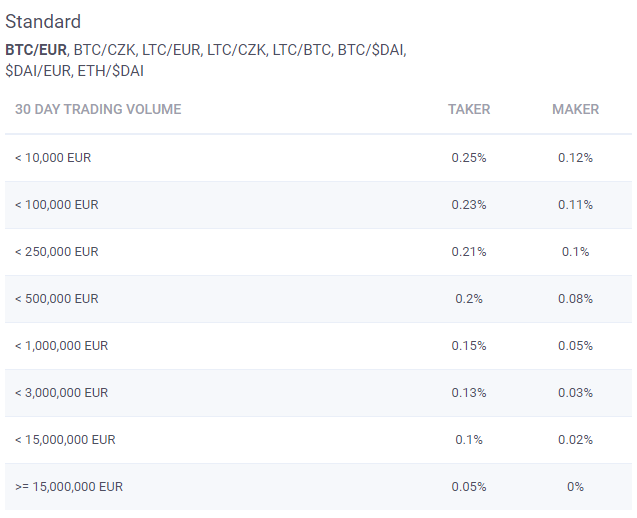
\includegraphics[width=1\textwidth]{images/coinmate_standard.PNG}
	\caption{Poplatky na burze Coinmate (taker - odběratel, maker - dodavatel) \cite{coinmate_fees}}\label{coinmate_standard}
\end{figure}
\begin{figure}\centering
	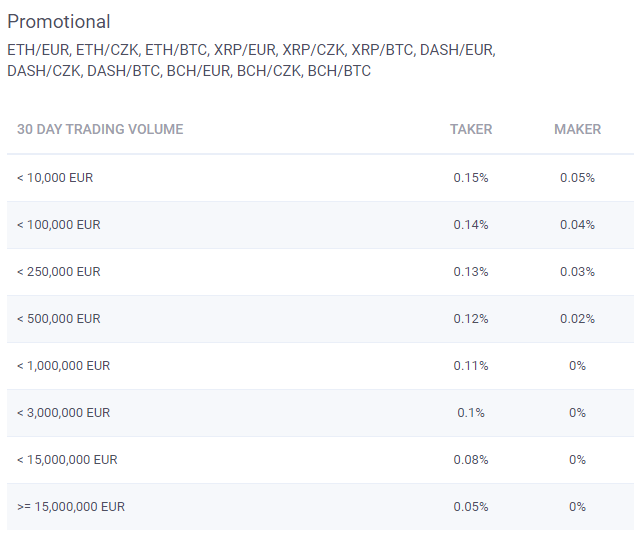
\includegraphics[width=1\textwidth]{images/coinmate_promotional.PNG}
	\caption{Poplatky na burze Coinmate (taker - odběratel, maker - dodavatel) \cite{coinmate_fees}}\label{coinmate_promotional}
\end{figure}
\subsection{Binance}
\paragraph{
Burza Binance byla založena v Číně v roce 2017, avšak později své sídlo přesunula na Maltu. Binance je podle dat z CoinMarketCap největší burzou, co se týče zobchodovaného objemu za posledních 30 dní. \cite{coinmarketcap} Burza podporuje obchodováním s 1320~odlišnými měnami, což silně převyšuje běžný standard.  
}
\paragraph{
Binance je také specifické tím, že všechny obchodovatelné dvojice se stávají pouze ze kryptoměn a ne běžných měn. Například americké dolary jsou nahrazeny stable coiny, jako je například USDT nebo TUSD. 
}
\paragraph{
Burza Binance si v průměru účtuje 0.1~\% za provedené obchody s měnami. Tento poplatek je stejný, jak pro dodavatele, tak i pro odběratele. Pokud se uživatel rozhodne zaplatit tyto poplatky domovskou měnou binance coin (BNB), pak jsou tyto poplatky redukovány o polovinu. Z toho plyne, že poplatky na burze Binance patří k jedněm z nejnižších.
}
\paragraph{
Co se týče výběrových a vkladových poplatků, tak vkladové poplatky jsou zadarmo pro veškeré měny. Na druhou stranu výběrové poplatky se liší pro každou měnu (viz \ref{binance_fees}). \cite{blockonomi_binance}
}
\begin{figure}\centering
    \begin{center}
     \begin{tabular}{||c | c | c | c||} 
     \hline
     Měna/token & Název & Minimální výběr & Výběrový poplatek \\ [0.5ex] 
     \hline\hline
     BTC & Bitcoin & 0,001 & 0,0004 \\ 
     \hline
     LTC & Litecoin & 0,002 & 0,001 \\
     \hline
     ETH & Ethereum & 0,02 & 0,003 \\
     \hline
     XMR & Monero & 0,0002 & 0,0001 \\
     \hline
     XRP & Ripple & 0,5 & 0,25 \\
     \hline
     BCH & Bitcoin Cash & 0,002 & 0,001 \\
     \hline
     EOS & EOS & 0,2 & 0,1 \\
     \hline
     BNB & BNB & 0,12 & 0 \\
     \hline
     TRX & TRON & 2,16 & 1,08 \\
     \hline
     USDT & TetherUS & 1,44 & 0,72 \\ [1ex] 
     \hline
    \end{tabular}
    \end{center}
    \caption{Výběrové poplatky na burze Binance \cite{binance_fees}}
    \label{binance_fees}
\end{figure}
\subsection{MXC}
\paragraph{
Burza MXC je jednou z novějších burz, která vznikla v dubnu roku 2018 a od svého vzniku je registrována v Singapuru. Podle statistik serveru CoinMarketCap je tato burza druhou největší z pohledu zobchodovatelného objemu za poslesdních 30 dní. \cite{coinmarketcap} MXC podobně jako burza Binance podporuje velké množství altcoinů, celkově je zde možné obchodovat s 264 měnami. \cite{mxc_coins}
}
\paragraph{
Burza se snaží nalákat uživatele na základě těchto tří propagovaných vlastností: velkým výkonem, super nodem a velmi pokročilým zabezpečením. Super node je distribuované decentralizované uložiště, které má zajistit adekvátní autonomii.
}
\paragraph{
Co se týče poplatků, patří burza MXC se svými poplatky o~velikosti 0,2~\% v průměru stále mezi nadprůměrné. Poplatek pro dodavatele i odběratele je totožný. Tím, že tato burza patří mezi špičku, co se týče zobchodovaného objemu, je tím zaručena i dostatečná likvidita. \cite{cryptowisser_mxc} 
}
\paragraph{
Burza MXC stejně jako Binance nezpoplatňuje vklad jakékoliv měny, zpoplatňuje také výběry jednotlivých měn. Tyto výběrové poplatky se mohou periodicky měnit na základě situace jednotlivých bloků. \cite{mxc_fees} Na základě tabulek \ref{mxc_fees} a \ref{binance_fees} je možné vidět, že jsou výběrové poplatky velmi podobné jako na burze Binance, jediný znatelný rozdíl je u TetherUS (USDT). \cite{cryptowisser_mxc}
}
\begin{figure}\centering
    \begin{center}
     \begin{tabular}{||c | c | c | c||} 
     \hline
     Měna/token & Název & Minimální výběr & Výběrový poplatek \\ [0.5ex] 
     \hline\hline
     BTC & Bitcoin & 0,001 & 0,0005 \\ 
     \hline
     LTC & Litecoin & 0,01 & 0,001 \\
     \hline
     ETH & Ethereum & 0,04 & 0,005 \\
     \hline
     XMR & Monero & 0,1 & 0,01 \\
     \hline
     XRP & Ripple & 50 & 0,1 \\
     \hline
     BCH & Bitcoin Cash & 0,02 & 0,001 \\
     \hline
     EOS & EOS & 2 & 0,1 \\
     \hline
     BNB & BNB & 0,3 & 0,001 \\
     \hline
     TRX & TRON & 600 & 1 \\
     \hline
     USDT & TetherUS & 25 & 4,8 \\ [1ex] 
     \hline
    \end{tabular}
    \end{center}
    \caption{Výběrové poplatky na burze MXC \cite{mxc_fees}}
    \label{mxc_fees}
\end{figure}
\subsection{BitForex}
\paragraph{
Burza BitForex je krytpoměnová burza, která vznikla v červnu roku 2018 a v dnešní době se podle serveru CoinMarketCap řadí dvanácté místo, co se týče obchodovaného objemu za posledních 30 dní. \cite{coinmarketcap} BitForex svým více jak 3 milionům uživatelům umožňuje obchodování na 92 měnových párech.  \cite{cryptowisser_bitforex}
}
\paragraph{
BitForex má oproti odhadovanému průměru (0,25~\%) velmi zajímavé poplatky, pouze 0,1~\% stejný pro dodavatele i odběratele. Burza BitForex se snaží cílit na větší obchodníky, a proto pro ty, kteří vlastní alespoň 50~bitcoinů v rámci burzy a k tomu mají obchodovatelný objem za posledních 30~dní alespoň 1000~bitcoinů (řádově jednotky milionů dolarů), poskytuje burza nulové poplatky. 
}
\paragraph{
BitForex nezpoplatňuje jakékoliv vklady jednotlivých kryptoměn, ale stejně jako Binance nebo MXC zpoplatňuje výběry víceméně podobnými poplatky (viz tabulka \ref{bitforex_fees}). \cite{cryptowisser_bitforex}
}

\begin{figure}\centering
    \begin{center}
     \begin{tabular}{||c | c | c | c||} 
     \hline
     Měna/token & Název & Minimální výběr & Výběrový poplatek \\ [0.5ex] 
     \hline\hline
     BTC & Bitcoin & 0,001 & 0,0005 \\ 
     \hline
     LTC & Litecoin & 0,1 & 0,001 \\
     \hline
     ETH & Ethereum & 0,01 & 0,02 \\
     \hline
     XMR & Monero & 0,01 & 0,00005 \\
     \hline
     XRP & Ripple & 20 & 0,15 \\
     \hline
     BCH & Bitcoin Cash & 0,012 & 0,0001 \\
     \hline
     EOS & EOS & 10 & 0,1 \\
     \hline
     BNB & BNB & 0,1 & 0,001 \\
     \hline
     TRX & TRON & 250 & 20 \\
     \hline
     USDT & TetherUS & 10 & 2 \\ [1ex] 
     \hline
    \end{tabular}
    \end{center}
    \caption{Výběrové poplatky na burze BitForex \cite{bitforex_fees}}
    \label{bitforex_fees}
\end{figure}

\subsection{LBank}
\paragraph{
LBank je kryptoměnová burza sídlící v Hong Kongu. Jedná se o jednu z největších burz, která se podle statistik z CoinMarketCap řadí v obchodovaném objemu za posledních 30~dní na deváté místo. \cite{coinmarketcap} \cite{cryptowisser_lbank}
}
\paragraph{
Co se týče poplatků, tak burza LBank využívá takzvaně plochý model poplatků, poplatky pro odběratele i dodavatele jsou totožné, ve výši 0,1~\%. Jedná se o nadprůměrně nízké poplatky. LBank je oproti svým konkurentům velmi zajímavá tím, že nezpoplatňuje ani vklad ani výběr jakýchkoliv měn. 
}
\paragraph{
Malou nevýhodou LBank je, že neumožňuje vklad pomocí kreditné karty. \cite{cryptowisser_lbank}
}

\section{Arbitrážní příležitosti}
\subsection{Efektivita trhu}
\paragraph{
Efektivní je takový trh, kdy jsou všechny dostupné informace zpracovávány a zohledněny v ceně aktiv (měn, akcií, dluhopisů, komodit). Na dokonale efektivním trhu ovlivňuje výnosnost jednotlivých investic pouze náhoda a není možné ji zlepšit za pomoci jakýchkoliv technických prostředků ani technickou analýzou. \cite{efektivita_trhu}
}
\paragraph{
Reálné trhy nikdy dokonale efektivní nejsou. Na těchto neefektivních trzích je pak možné sledovat arbitrážní příležitosti, které vznikají právě z neefektivity trhu. \cite{what_is_arbitage}
}
\subsection{Arbitráž}
\paragraph{
Arbitráž je obchodní strategie, která má za cíl vytěžit na neefektivitě trhu. Arbitráž je založena na principu nakoupit levně a prodat draze. Principem arbitráže je vytvořit zisk na malých rozdílech v ceně aktiv. Nejčastěji se jedná o nákup na jednom místě a téměř instantní prodej na místě jiném za vyšší cenu. \cite{Capital}
}
\subsection{Arbitráže v rámci kryptoměnových burz}
\paragraph{
Arbitrážní příležitost vznikne většinou na základě rozdílu cen na dvou odlišných burzách. Důvod proč arbitráže vznikají právě na kryptoměnových burzách je ten, že na burzách, kde dochází k velkému obchodnímu objemu, vzniká i velká likvidita určité měny, která poté reaguje rychleji na změny cen. Zatímco na burzách, kde je menší nabídka dané měny, je likvidita nižší a cena dané měny bude daleko pomaleji reagovat na změny. Tím, že je možné nakoupit na jedné burze levněji a na druhé prodat dráže, vznikne neefektivita a s ní také potenciální zisk.
}
\paragraph{
Tento efekt velice úzce souvisí s tím, že se kryptoměny staly v posledních letech velmi populárními a ceny na velkých burzách velmi rychle kolísají, zatímco menší burzy tomuto tempu nemusí vždy stíhat. \cite{finder}
}

\subsection{Měnový pár v rámci kryptoměnových burz}
\paragraph{
Měnový pár je vztah mezi dvěma měnami určující hodnotu jedné vůči druhé. Například USD/CZK je vztah dolaru vůči koruně. První uváděná měna je vždy označována jako základní měna, zatímco druhá měna se označuje jako kótovaná měna. \cite{Capital_menovy_par} 
} 
\paragraph{
Poměr je uváděn ve vztahu k základní měně. Pokud je nákupní cena USD/CZK 22,5, znamená to, že je možné nakoupit 1~dolar za 25,5~ Korun českých. Běžně je uváděn i otočený kurz tedy CZK/USD. \cite{Capital_menovy_par} 
}
\paragraph{
V rámci kryptoměnových burz je běžné uvádět pouze jeden kurz například LTC/BTC, ne však otočený BTC/LTC. Z toho důvodu jsou na kryptoměnových burzách u jednotlivých kurzů vždy uváděny dvě hodnoty bid (nabídka) a ask (poptávka). 
}
\paragraph{
V rámci kryptoměnových burz se značení mezi měnovými páry často liší, avšak většinou se používá jedna z těchto tří možností (AAA/BBB, AAA-BBB, AAABBB), kde AAA a BBB zastupují zkratku nějaké měny (kryptoměny).
}
\subsection{Deterministické arbitrážní příležitosti}
\paragraph{
Deterministické arbitráže jsou základním typem arbitrážních příležitostí, které mohou vznikat na kryptoměnových burzách. Jedná se o nákup a prodej stejných měnových párů na různých burzách v co nejkratším časovém intervalu za účelem výdělku. \cite{CZInvestor} \cite{TowardsDataScience}
}
\paragraph{
Například nakoupím v jednom čase litecoin na burze Binance za 38,31~\$ a co nejrychleji prodám na burze Coinmate za 38,70~\$ a tím vydělám 0,39~\$. Toto je nejjednodušší příklad a neberu zatím v potaz poplatky, které mají jednotlivé burzy zavedené. 
}
\subsection{Trojúhelníkové arbitrážní příležitosti}
\paragraph{
Trojúhelníková arbitráž na kryptoměnových burzách je takový obchod, kdy dojde k nákupu a prodeji mezi třemi měnami za cílem zisku. K této arbitráži může docházet, buď v rámci jedné burzy nebo mezi několika odlišnými (v následující části se budu věnovat arbitrážní příležitosti na jedné burze). \cite{TradingStrategy}
}
\paragraph{
Cílem je mít nějakou obchodovatelnou měnu A, tu směníme na měnu B, tu následně na měnu C a nakonec opět zpátky na původní měnu A. Pokud máme měny A na konci více než na začátku, je možné detekovat arbitrážní příležitost. Tento efekt je způsoben neefektivností burzy.
}
\paragraph{
Příklad trojúhelníkové arbitrážní příležitosti: na burze jsou sledovanými páry LTCBTC, LTCETH, ETHBTC. V prvním kroku nakoupím za 1~bitcoin odpovídající množství litecoinů (podle LTCBTC). Toto množství v dalším kroku prodám za odpovídající množství etherea (podle LTCETC) a za zakoupenou sumu etherea koupím znovu bitcoin (podle ETHBTC). Pokud mám na konci více než bitcoinů, než kolik do trojúhelníku vstoupilo, vydělal jsem rozdíl mezi těmito dvěma obnosy (viz obr. \ref{triangle_arbitrage}).
}
\begin{figure}\centering
	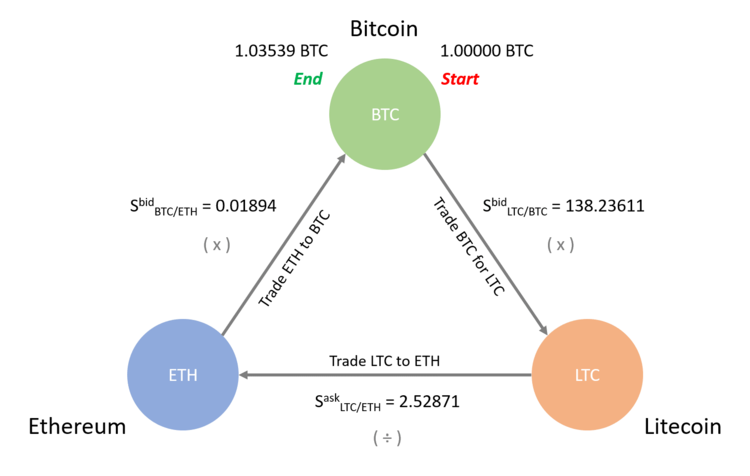
\includegraphics[width=1\textwidth]{images/ZMENIT-triangle.png}
	\caption{Trojúhelníková arbitráž}\label{triangle_arbitrage}
\end{figure}
\paragraph{
V rámci arbitrážních příležitostí je také nutné brát v potaz nákupní poplatky, které si burzy za každý nákup účtují. Tyto poplatky mohou být pro všechny dvojice stejné nebo se mohou pro každou obchodovatelnou dvojici lišit.  
}
\subsection{Problémy s vytěžováním arbitrážních příležitostí}
\paragraph{
O arbitrážních příležitostech se většinou mluví jako o obchodech bez rizika. Existují však nějaké bariéry a rizika, která je nutné brát v potaz.
}
\paragraph{
Jedním z prvních problémů mohou být takzvané KYC regulace (know your customer - poznej svého zákazníka). Tyto regulace mohou například omezovat to, že pro obchodování na burze je nutné mít bankovní účet v zemi, kde je burza situována.
}
\paragraph{
Kvůli tomu, že procentuální zisk arbitrážních příležitostí je většinou velmi nízký, je nutné provést obchod ve velké sumě. Z toho plyne, že je nutné mít poměrně velký obnos kryptoměn uložen na jednotlivých burzách kvůli tomu, aby bylo možné provést obchod co nejrychleji po detekci arbitrážní příležitosti. 
}
\paragraph{
Poplatky mezi obchody na burzách mohou výrazně snížit potenciální zisk a i po detekci neefektivity trhu nemusí nutně dojít k okamžitému výdělku.  
}
\paragraph{
Dalším problémem je, že se vůbec nemusí podařit provést transakci dostatečně rychle na to, aby ji neprovedl někdo jiný. Tím pádem se vždy nemusí podařit vytěžit arbitrážní příležitost nebo může proběhnout pouze část transakcí, které mohou skončit v záporných číslech.
}
\paragraph{
Na některých burzách se objevovaly i problémy s pomalým proběhnutím transakcí, které mohly také způsobit určitou ztrátu, pokud je někdo závislý na rychlém pohybu mezi kryptoměnami. \cite{finder}
}
\chapter{Realizace}
\paragraph{
V této sekci se zabývám praktickou částí své bakalářské práce, ve které se ze začátku zaměřuji na problémy se získáváním relevantních dat. Dále na to navazuji záznamem o svém počínání v rámci analýzy těchto získaných dat. 
}
\paragraph{
V poslední podkapitole se poté věnuji praktickým výstupům své práce, zejména statistikám o mých úspěších z vytěžování reálných arbitrážních příležitostí a na to navazujícím výpočetem týkající se toho, jak moc je výhodné se prakticky snažit vytěžovat tyto příležitosti.
}
\section{Získání dat}
\paragraph{
V této kapitole se zaměřuji na problémy, na které jsem narazil při získávání dat. Zabývám se zde také dostupností dat na jednotlivých burzách či jiných serverech, které tata data poskytují. 
}
\paragraph{
Obecně jsem potřeboval  taková data, která by mi byla schopna poskytnout informaci v konkrétním čase, týkající se aktuálních nabídek a poptávek pro jednotlivé dvojice měn, na kterých jsem chtěl provádět analýzu.
}
\subsection{Data na kryptoměnových burzách}
\paragraph{
Nejdříve jsem se snažil získat data na oficiálních stránkách jednotlivých burz, konkrétně binance.com, kraken.com a cryptowatch.com. Zde jsem se byl schopen po registraci připojit na jednotlivá api. Data zde byla veřejně k dispozici, avšak neodpovídala takovému formátu, který jsem pro svou práci požadoval. 
}
\paragraph{
Na všech kryptoměnových burzách byla k dispozici data pouze o aktuálních nabídkách a poptávkách. Co se týče historických dat, tak bylo možné získat data o všech provedených obchodech, kde bylo vždy uvedeno minimálně množství, cena a čas provedení obchodu. Dále bylo možné získat data k vytvoření svícnových grafů. Všechna tato historická data byla pro mě však irelevantní. 
}
% todo - doplnit citace na jednotlivé burzy
\subsection{Burza Binance}
\paragraph{
Jako burzu, ze které jsem sbíral data, jsem si vybral server Binance. Tuto burzu jsem si vybral především z toho důvodu, že zde probíhá nejvíce obchodů, co se týče zobchodovaného objemu. Podle serveru CoinMarketCap je zde zobchodováno minimálně o 50~\% objemu více (objem za posledních 30 dní) než na jakékoli jiné burze. \cite{coinmarketcap}
}
\paragraph{
Dalšími podpůrnými parametry pro výběr této burzy bylo to, že měla přívětivé api, a dalo se na ni připojit jednoduše přes websocket. \cite{BinanceApi}
}
\subsection{Vlastní sběr dat}
\paragraph{
Z důvodu, že jsem nebyl schopen nikde sehnat odpovídající data, která jsem potřeboval pro svou práci, byl přinucen si data začít sbírat z burz sám.
}
\paragraph{
K Binance api jsem se připojil přes websocket, přes který mi při každé změně chodila data ohledně aktuální nabídky a poptávky sledované dvojice měn. Tato data jsem si vždy ihned uložil včetně aktuálního časového záznamu ve formátu unix timestamp.\cite{BinanceApi}
}
\paragraph{
Neboť jsem data potřeboval ukládat pořád a ne pouze v konkrétní časové intervaly, tak jsem sběr dat spustil na cloudové službě AWS - Amazon Web Services. Data jsem kumuloval do souborů po jednom dni, protože jsem kvůli omezenému uložišti musel data stahovat a ukládat i na lokální disk.
}
\subsubsection{Sledované měny}
\paragraph{
Na serveru Binance je možné obchodovat s 1320 různými měnami (údaj k 29.3. 2020). Protože pro mě nebylo reálné sledovat tolik různých dvojic, vybral jsem si ke sledování následující měny: USDT, BTC, LTC, ETH, XRP, BCH, EOS, BNB, TRX, XMR. Což celkově znamenalo sbírat data týkající se 39 dvojic (obchody mezi některými dvojicemi na severu Binance nebylo možné provádět). Všechna tato data nabývala velikosti v průměru téměř 1 GB za den.
}
% todo - napsat názvy měn
\section{Zpracování dat}
\paragraph{
V této podkapitole se budu věnovat tématu se zpracováním nasbíraných dat.
}
\subsection{Filtrování surových dat}
\paragraph{
V prvním kroku bylo mým cílem pouze vyfiltrovat všechny potenciální arbitrážní příležitosti, které mohli nastat. Potenciální z toho důvodu že jsem ještě nebral v potaz poplatky, kterými Binance zpoplatňuje kažný provedený obchod.
}
\paragraph{
Nejdříve jsem tento filtrovací skript napsal v jazyce Python. Zde však probíhalo filtrování moc pomalu. Z toho důvodu jsem výběr Pythonu přehodnotil a rozhodl jsem se využít jazyka C++. 
}
\paragraph{
V jazyce C++ se mi podařilo filtrování zrychlit téměř šedesátkrát. Vyfiltrovaná data jsem nyní ukládal v JSON formátu. Tento formát jsem si vybral z toho důvodu, že je zde možné přehledněji strukturovat data. Ukládal jsem si do těchto souborů například i informace o tom, jaké konkrétní obchody jsou nejvýhodnější, jaký teoretický zisk mohl nastat. 
}
\begin{figure}\centering
	
\includegraphics[width=1\textwidth]{images/placeholder.png}
	\caption{Ukázka JSON formátu struktury dat}\label{fig:pokus}
\end{figure}
%\ref{fig:gnuplot-col}
% todo - změnit obrázek na JSON example
\subsection{Arbitrážní příležitosti}
\paragraph{
Ve své práci se věnuji pouze arbitrážním příležitostem pro 3 různé měny. Protože mám pro libovolnou obchodovatelnou dvojici kryptoměn (AAA a BBB) vždy údaj pouze z jedné strany (poptávka i nabídka je pouze z pohledu jedné z kryptoměn) může docházet v trojúhelníku k následujícím možnostem (viz tabulka \ref{tabulka_kombinaci}). Těchto osm možností je však možné pouhým přeházením dostat do dvou odlišných kombinací (viz zelené a modré možnosti v tabulce \ref{tabulka_kombinaci}).
}
\begin{figure}\centering
	\includegraphics[width=1\textwidth]{images/tabulka_kombinací.PNG}
	\caption{Tabulka různých kombinací trojúhelníků}\label{tabulka_kombinaci}
\end{figure}
\paragraph{
Z výsledných dvou různých kombinací je ještě nutné rozlišit, jakým způsobem bude docházet k detekci arbitrážní příležitosti. To je opět naznačeno pomocí znaků dělena ('/') a násobení ('*') a pomocí barev v tabulce \ref{2_kombinace}. Tato tři čísla se mezi sebou vždy příslušně vynásobí nebo vydělí a pokud je výsledné číslo vyšší než 1, pak je detekována potenciální arbitrážní příležitost. 
}
\paragraph{
Dalším krokem v rámci detekce ideální příležitosti je projití několika dalších nejlepších nabídek (poptávek), v mém případě celkem pěti, a zjišťovat, jestli není výhodnější provést obchod s menším procentuálním ziskem, avšak s vyšším absolutním ziskem. Snažím se tedy najít takovou možnost, při které dojde k zobchodování většího množství a tím vznikne vyšší zisk.
}

\begin{figure}\centering
	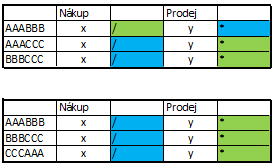
\includegraphics[width=0.5\textwidth]{images/2_kombinace.PNG}
	\caption{Odlišné způsoby detekce arbitrážních příležitostí}\label{2_kombinace}
\end{figure}

\begin{conclusion}
\paragraph{
V práci jsem zatím úspěšně naimplementoval program v programovacím jazyce Python, který se stará o sběr dat. Tento program jsem nasadil na cloudovou službu Amazon Web Services, kde běží bez přerušení. 
}
\paragraph{
V teoretické části jsem zatím napsal velmi stručnou rešerši, kterou mám ještě v plánu značně rozšiřovat. Našel jsem si již zdroje i k následujícím částem teoretické části.  Plánuji se zde ještě více věnovat kryptoměnám podrobněji a popsat více jejich charakteristiky. Dále zde plánuji zpracovat rešerši týkající se dosavadních prací, které se také zabývají otázkou arbitrážních příležitostí.
}
\paragraph{
Mým dalším krokem je napsání programu, který bude analyzovat nasbíraná data. Na tomto úkolu mohu pracovat i s prozatímními daty, neboť se na programu nic nezmění, pouze se změní výstupní statistiky. Tato část bude stěžejní částí mé celkové bakalářské práce.
}
\paragraph{
Úplně nakonec se budu věnovat výstupům, které zjistím v části analýzy dat. Tyto data zpracuji jako celek a zaměřím se na výstupy, které je možné na datech pozorovat.
}

\end{conclusion}

\bibliographystyle{csn690}
\bibliography{mybibliographyfile}

\appendix

\chapter{Seznam použitých zkratek}
% \printglossaries
\begin{description}
	\item[GUI] Graphical user interface
	\item[XML] Extensible markup language
\end{description}


% % % % % % % % % % % % % % % % % % % % % % % % % % % % 
% % Tuto kapitolu z výsledné práce ODSTRAŇTE.
% % % % % % % % % % % % % % % % % % % % % % % % % % % % 
% 
% \chapter{Návod k~použití této šablony}
% 
% Tento dokument slouží jako základ pro napsání závěrečné práce na Fakultě informačních technologií ČVUT v~Praze.
% 
% \section{Výběr základu}
% 
% Vyberte si šablonu podle druhu práce (bakalářská, diplomová), jazyka (čeština, angličtina) a kódování (ASCII, \mbox{UTF-8}, \mbox{ISO-8859-2} neboli latin2 a nebo \mbox{Windows-1250}). 
% 
% V~české variantě naleznete šablony v~souborech pojmenovaných ve formátu práce\_kódování.tex. Typ může být:
% \begin{description}
% 	\item[BP] bakalářská práce,
% 	\item[DP] diplomová (magisterská) práce.
% \end{description}
% Kódování, ve kterém chcete psát, může být:
% \begin{description}
% 	\item[UTF-8] kódování Unicode,
% 	\item[ISO-8859-2] latin2,
% 	\item[Windows-1250] znaková sada 1250 Windows.
% \end{description}
% V~případě nejistoty ohledně kódování doporučujeme následující postup:
% \begin{enumerate}
% 	\item Otevřete šablony pro kódování UTF-8 v~editoru prostého textu, který chcete pro psaní práce použít -- pokud můžete texty s~diakritikou normálně přečíst, použijte tuto šablonu.
% 	\item V~opačném případě postupujte dále podle toho, jaký operační systém používáte:
% 	\begin{itemize}
% 		\item v~případě Windows použijte šablonu pro kódování \mbox{Windows-1250},
% 		\item jinak zkuste použít šablonu pro kódování \mbox{ISO-8859-2}.
% 	\end{itemize}
% \end{enumerate}
% 
% 
% V~anglické variantě jsou šablony pojmenované podle typu práce, možnosti jsou:
% \begin{description}
% 	\item[bachelors] bakalářská práce,
% 	\item[masters] diplomová (magisterská) práce.
% \end{description}
% 
% \section{Použití šablony}
% 
% Šablona je určena pro zpracování systémem \LaTeXe{}. Text je možné psát v~textovém editoru jako prostý text, lze však také využít specializovaný editor pro \LaTeX{}, např. Kile.
% 
% Pro získání tisknutelného výstupu z~takto vytvořeného souboru použijte příkaz \verb|pdflatex|, kterému předáte cestu k~souboru jako parametr. Vhodný editor pro \LaTeX{} toto udělá za Vás. \verb|pdfcslatex| ani \verb|cslatex| \emph{nebudou} s~těmito šablonami fungovat.
% 
% Více informací o~použití systému \LaTeX{} najdete např. v~\cite{wikilatex}.
% 
% \subsection{Typografie}
% 
% Při psaní dodržujte typografické konvence zvoleného jazyka. České \uv{uvozovky} zapisujte použitím příkazu \verb|\uv|, kterému v~parametru předáte text, jenž má být v~uvozovkách. Anglické otevírací uvozovky se v~\LaTeX{}u zadávají jako dva zpětné apostrofy, uzavírací uvozovky jako dva apostrofy. Často chybně uváděný symbol "{} (palce) nemá s~uvozovkami nic společného.
% 
% Dále je třeba zabránit zalomení řádky mezi některými slovy, v~češtině např. za jednopísmennými předložkami a spojkami (vyjma \uv{a}). To docílíte vložením pružné nezalomitelné mezery -- znakem \texttt{\textasciitilde}. V~tomto případě to není třeba dělat ručně, lze použít program \verb|vlna|.
% 
% Více o~typografii viz \cite{kobltypo}.
% 
% \subsection{Obrázky}
% 
% Pro umožnění vkládání obrázků je vhodné použít balíček \verb|graphicx|, samotné vložení se provede příkazem \verb|\includegraphics|. Takto je možné vkládat obrázky ve formátu PDF, PNG a JPEG jestliže používáte pdf\LaTeX{} nebo ve formátu EPS jestliže používáte \LaTeX{}. Doporučujeme preferovat vektorové obrázky před rastrovými (vyjma fotografií).
% 
% \subsubsection{Získání vhodného formátu}
% 
% Pro získání vektorových formátů PDF nebo EPS z~jiných lze použít některý z~vektorových grafických editorů. Pro převod rastrového obrázku na vektorový lze použít rasterizaci, kterou mnohé editory zvládají (např. Inkscape). Pro konverze lze použít též nástroje pro dávkové zpracování běžně dodávané s~\LaTeX{}em, např. \verb|epstopdf|.
% 
% \subsubsection{Plovoucí prostředí}
% 
% Příkazem \verb|\includegraphics| lze obrázky vkládat přímo, doporučujeme však použít plovoucí prostředí, konkrétně \verb|figure|. Například obrázek \ref{fig:float} byl vložen tímto způsobem. Vůbec přitom nevadí, když je obrázek umístěn jinde, než bylo původně zamýšleno -- je tomu tak hlavně kvůli dodržení typografických konvencí. Namísto vynucování konkrétní pozice obrázku doporučujeme používat odkazování z~textu (dvojice příkazů \verb|\label| a \verb|\ref|).
% 
% \begin{figure}\centering
% 	
\includegraphics[width=0.5\textwidth, angle=30]{cvut-logo-bw}
% 	\caption[Příklad obrázku]{Ukázkový obrázek v~plovoucím prostředí}\label{fig:float}
% \end{figure}
% 
% \subsubsection{Verze obrázků}
% 
% % Gnuplot BW i barevně
% Může se hodit mít více verzí stejného obrázku, např. pro barevný či černobílý tisk a nebo pro prezentaci. S~pomocí některých nástrojů na generování grafiky je to snadné.
% 
% Máte-li například graf vytvořený v programu Gnuplot, můžete jeho černobílou variantu (viz obr. \ref{fig:gnuplot-bw}) vytvořit parametrem \verb|monochrome dashed| příkazu \verb|set term|. Barevnou variantu (viz obr. \ref{fig:gnuplot-col}) vhodnou na prezentace lze vytvořit parametrem \verb|colour solid|.
% 
% \begin{figure}\centering
% 	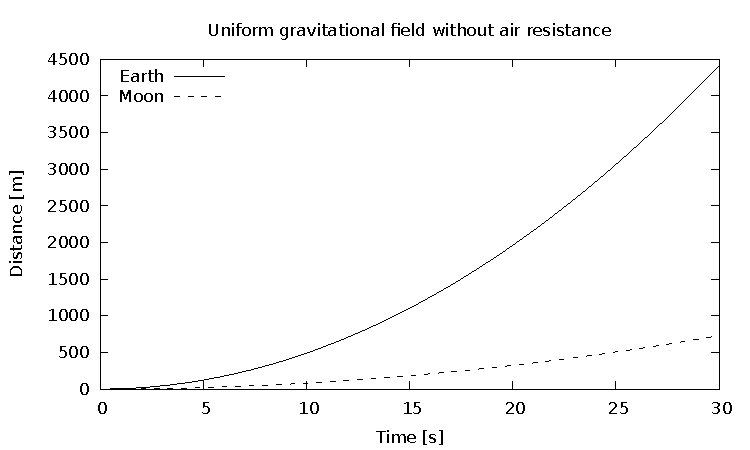
\includegraphics{gnuplot-bw}
% 	\caption{Černobílá varianta obrázku generovaného programem Gnuplot}\label{fig:gnuplot-bw}
% \end{figure}
% 
% \begin{figure}\centering
% 	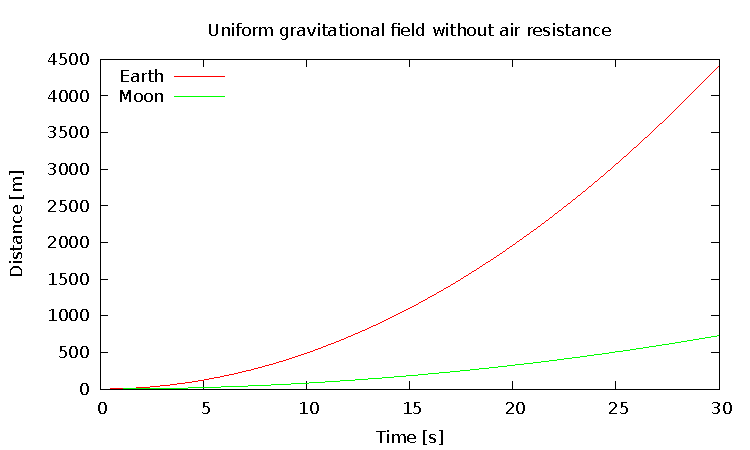
\includegraphics{gnuplot-col}
% 	\caption{Barevná varianta obrázku generovaného programem Gnuplot}\label{fig:gnuplot-col}
% \end{figure}
% 
% 
% \subsection{Tabulky}
% 
% Tabulky lze zadávat různě, např. v~prostředí \verb|tabular|, avšak pro jejich vkládání platí to samé, co pro obrázky -- použijte plovoucí prostředí, v~tomto případě \verb|table|. Například tabulka \ref{tab:matematika} byla vložena tímto způsobem.
% 
% \begin{table}\centering
% 	\caption[Příklad tabulky]{Zadávání matematiky}\label{tab:matematika}
% 	\begin{tabular}{|l|l|c|c|}\hline
% 		Typ		& Prostředí		& \LaTeX{}ovská zkratka	& \TeX{}ovská zkratka	\tabularnewline \hline \hline
% 		Text		& \verb|math|		& \verb|\(...\)|	& \verb|$...$|		\tabularnewline \hline
% 		Displayed	& \verb|displaymath|	& \verb|\[...\]|	& \verb|$$...$$|	\tabularnewline \hline
% 	\end{tabular}
% \end{table}
% 
% % % % % % % % % % % % % % % % % % % % % % % % % % % % 

\chapter{Obsah přiloženého CD}

%upravte podle skutecnosti

\begin{figure}
	\dirtree{%
		.1 readme.txt\DTcomment{stručný popis obsahu CD}.
		.1 exe\DTcomment{adresář se spustitelnou formou implementace}.
		.1 src.
		.2 impl\DTcomment{zdrojové kódy implementace}.
		.2 thesis\DTcomment{zdrojová forma práce ve formátu \LaTeX{}}.
		.1 text\DTcomment{text práce}.
		.2 thesis.pdf\DTcomment{text práce ve formátu PDF}.
		.2 thesis.ps\DTcomment{text práce ve formátu PS}.
	}
\end{figure}

\end{document}